\documentclass{article}
\usepackage{fullpage}
\usepackage{hyperref}
\usepackage{graphicx} % new way of doing eps files
\usepackage{caption}
\usepackage{subcaption}
\usepackage{listings} % nice code layout
\usepackage[usenames]{color} % color
\definecolor{listinggray}{gray}{0.9}
\definecolor{graphgray}{gray}{0.7}
\definecolor{ans}{rgb}{1,0,0}
\definecolor{blue}{rgb}{0,0,1}
% \Verilog{title}{label}{file}
%for general listings, white on the inside
\lstset{language=C++}
\lstset{rulecolor=\color{blue}}
\lstset{linewidth=\textwidth}
\lstset{commentstyle=\textit, stringstyle=\upshape,showspaces=false}
\lstset{frame=tb}
%\lstset{literate={\ \ }{{\ }}1}
\lstset{basicstyle = \small}
\lstset{breaklines=true}
\lstset{postbreak=\mbox{\textcolor{red}{$\hookrightarrow$}\space}}

\newcommand{\Cpp}[3]{
  \lstset{language=C++}
  \lstset{backgroundcolor=\color{listinggray},rulecolor=\color{blue}}
  \lstset{linewidth=\textwidth}
  \lstset{commentstyle=\textit, stringstyle=\upshape,showspaces=false}
  \lstset{frame=tb}
  \lstset{literate={\ \ }{{\ }}1}
  \lstset{basicstyle = \small}
  \lstset{breaklines=true}
  \lstset{postbreak=\mbox{\textcolor{red}{$\hookrightarrow$}\space}}
  \lstinputlisting[caption={#1},label={#2}]{#3}
}


\author{Jackson Farley, Ellie Langley, and Erik Leinen}
\title{Smart Walker Project}


\begin{document}
\maketitle
\tableofcontents
\listoffigures


\section{Project Summary}
This device is implemented on a smart walker and determines whether the walker is being used and at what time. When not in use, the device gently reminders the user to use the walker, and when the gentle reminder fails, the harsh reminder is enacted. As more and more elderly use walking aids, and as the elderly population is more susceptible to injurious falls, it is difficult for an elderly person to achieve independence safely. This device will allow the elderly who require walking aids to live by themselves safely.

This device utilizes sensors to detect human presence on the upper and lower part of the walker. Depending on whether a human presence has been detected from the lower sensor, the upper sensor will then take a measurement. If the upper sensor has also taken a measurement with a proximal signal, then the device will output a “gentle reminder” by lighting the LED modules on the walker a solid yellow. If the walker has still not been used, then the device will output a “strong” reminder by flashing the LEDs red. When the buttons on the walker are pressed, the walker will go to an “in use state”. A time stamp will be taken using a clock module and output to the SD card module. 

Most of the electrical parts for the smart walker have been placed within a plastic, red Sparkfun box, with holes drilled for wires which need to go outside the box. The two push buttons have been placed on the handlebars of the walker. The device is powered by one 9V battery.

\subsection{Objectives}
The end objectives of this project are listed below. Some of the objectives are outside the scope of the immediate project, but the design process took place with all of these in mind, so they are all listed here. The final item on the list was specific to our implementation, and is therefore marked separately. 
\begin{itemize}
	\item \textbf{Accurately Analyze Human Interaction with the Walker}: Use two sensors to detect the presence of the user effectively, as well as have two buttons that detect whether the user is gripping the handles
	\item \textbf{Accurate Time Recording}: Have a real-time clock that is able to keep time even when the system is powered off
	\item \textbf{Notification}: Succesfully notify users when they are not using the walker and should. To do this we must have sufficient display capability and accurate analysis as explained above. The item should also be able to notify others if there is an emergency
	\item \textbf{Tracking}: The item should be able to record when the user has begun using the walker and keep that information for later analysis. Potentially an end objective would be creating a use-profile, so a doctor could be notified if there were significant deviations from this 
	\item \textbf{Portability}: An older person should be able to transport this as easily as his/her standard walker. It should easily fit in the back of a small car and not add to the bulk of the system
	\item \textbf{Low Cost}: This system, when fully deployed, should be inexpensive (under \$100, ideally under \$50)
	\item \textbf{Modularity}: The system should attach to the user's existing walker with very little setup and no power tools. 
	\item \textbf{Low Power}: The system should continue to work for at least 24 hours of normal operation on a single charge
	\item[\textasteriskcentered] \textbf{Relative Hardware Independence}: The code should work with potential changes in sensor or code with as little alteration as possible, therefore the functions and the objects to be interchangeable with a small amount of work where possible
\end{itemize}

\section{Hardware Design}
Before the current development team inherited the project, there was a significant amount of hardware that was already purchased that we chose from to make this project work. 

\subsection{Hardware Platform}
The Arduino Mega 2560 was selected as the hardware platform, as the sensors purchased for the project best interface with the Arduino family due to large libraries. This is also what the previous developers had been using and was readily available for low cost. Additionally, the added capability over the Arduino Uno gave greater flexibility and resources for computing once our system became much larger.  

Other useful features include: 
\begin{itemize}
	\item Quick Up-Time: The Mega, once turned on, is ready in a matter of seconds, which allows it to record initial use and reduce potential annoyance to users. While it is designed to be on all the time, it is also good to know that the device won't break or fry if there is a sudden loss of power. 
	\item Lower Power: The Beaglebone, while much more capable than the Mega, consumed much more power than the mega, meaning it would require a heavy and expensive battery to continue operation for the objective amount of time. 
	\item Configurable Interrupts: the buttons implemented in this project must be configured as interrupts for the purpose of the device to be achieved. 
	\item I$^2$C: many sensors communicate via this protocol, including some of the QWIIC enabled components by Sparkfun like the Real-Time Clock and the RF sensor. 
\end{itemize}

\subsection{Schematic}

The schematic is shown below in Figure~\ref{fig:schematic}. It depicts the basic elements used and pins used on the Arduino Mega.

\begin{figure} [h]
	\begin{center}
		\caption {The Schematic} \label{fig:schematic}
		\includegraphics[width=\textwidth]{./images/schematic.png}
	\end{center}
\end{figure}

The microcontroller used was the Arduino Mega 2560, and the Arduino IDE was used to implement the code onto the board. An Arduino Mega Protoshield was used to make the middle connections needed to reach the same circuit as shown in Figure 1. The proto board had the resistors and capacitors soldered onto it so that a hardware debounce was created for the buttons to give the most accurate readings of the button press. Above the protoshield, was another Wi-Fi shield that will be used in future developments of this product to help implement the ability to store data onto a website that can be accessed by another device. The Arduino is powered by a 9V battery, but in the future, it is desired that a rechargeable battery substitute should be used.
 
The LED modules used for the display of the states use 3.3V logic in order to operate and have four different pins. The voltage in, the ground, the SCL, and the SDA pins. They are powered by the 3.3V pin on the Arduino Mega, and connected to the SCL and SDA pins as well. The next connection is the QWIIC adapter module. This was used to connect multiple QWIIC compatible devices together without having to connect separate wires from the SDA and SCL pins. This reduced wires and made packaging easier. All QWIIC components use 3.3V logic and are therefore connected to the 3.3V pin on the Arduino. Connected to the QWIIC adapter is the RF Time of Flight Sensor, and the Real Time Clock. Both devices were connected through the QWIIC wiring, and only have those connections used. The Real Time clock has a small battery that charges when power is applied to the board, and expends power from the battery when there is no power in. This allows the module to keep track of the current time even if the power is removed. The next module used was the Shifting Micro SD Breakout, which was used to write the data onto a micro SD card. For the Arduino Mega, the SCK, DI, and D0 pins must be connected exactly to digital pins 52, 51, and 50 respectively. The CS pin and CD pin can be connected to any other digital pin, but it was decided to use digital pins 8 and 9 for this project. This module is the only one that requires 5V logic and is therefore connected to the 5V pin to the Arduino. The last module is the Open PIR Sensor. This uses 3.3V logic and outputs a digital and analog signal, but only the digital output is needed for this project. 

One other module that would be nice to include is a speaker, that would output an audible noise for different states to grab the attention of the user. This was not implemented due to time constraints but is a goal of the project sponsor.

\subsection{Parts Used}
The specific hardware components are listed below. Additionally, the URLs of where many components can be purchased are given in the Appendices. All of these components were combined into a Sparkfun Big Red Box, as shown in Figure~\ref{fig:completeWalker}. The lid off of the box to reveal the internal components is shown in Figure~\ref{fig:lidoff}. The Full Labeled System image is found in Figure~\ref{fig:labels} on Page~\pageref{fig:labels} in the Appendices.  



\begin{figure} [h!]
	\centering
	\begin{minipage}{.5\textwidth}
		\centering
		\caption {The Inside of the Big Red Box} \label{fig:lidoff}
		\includegraphics[width=.6\textwidth, angle=270]{./images/uncoveredBox.jpg}
	\end{minipage}%
	\begin{minipage}{.5\textwidth}
		\centering
		\caption {The Box Mounted onto the Walker} \label{fig:completeWalker}
		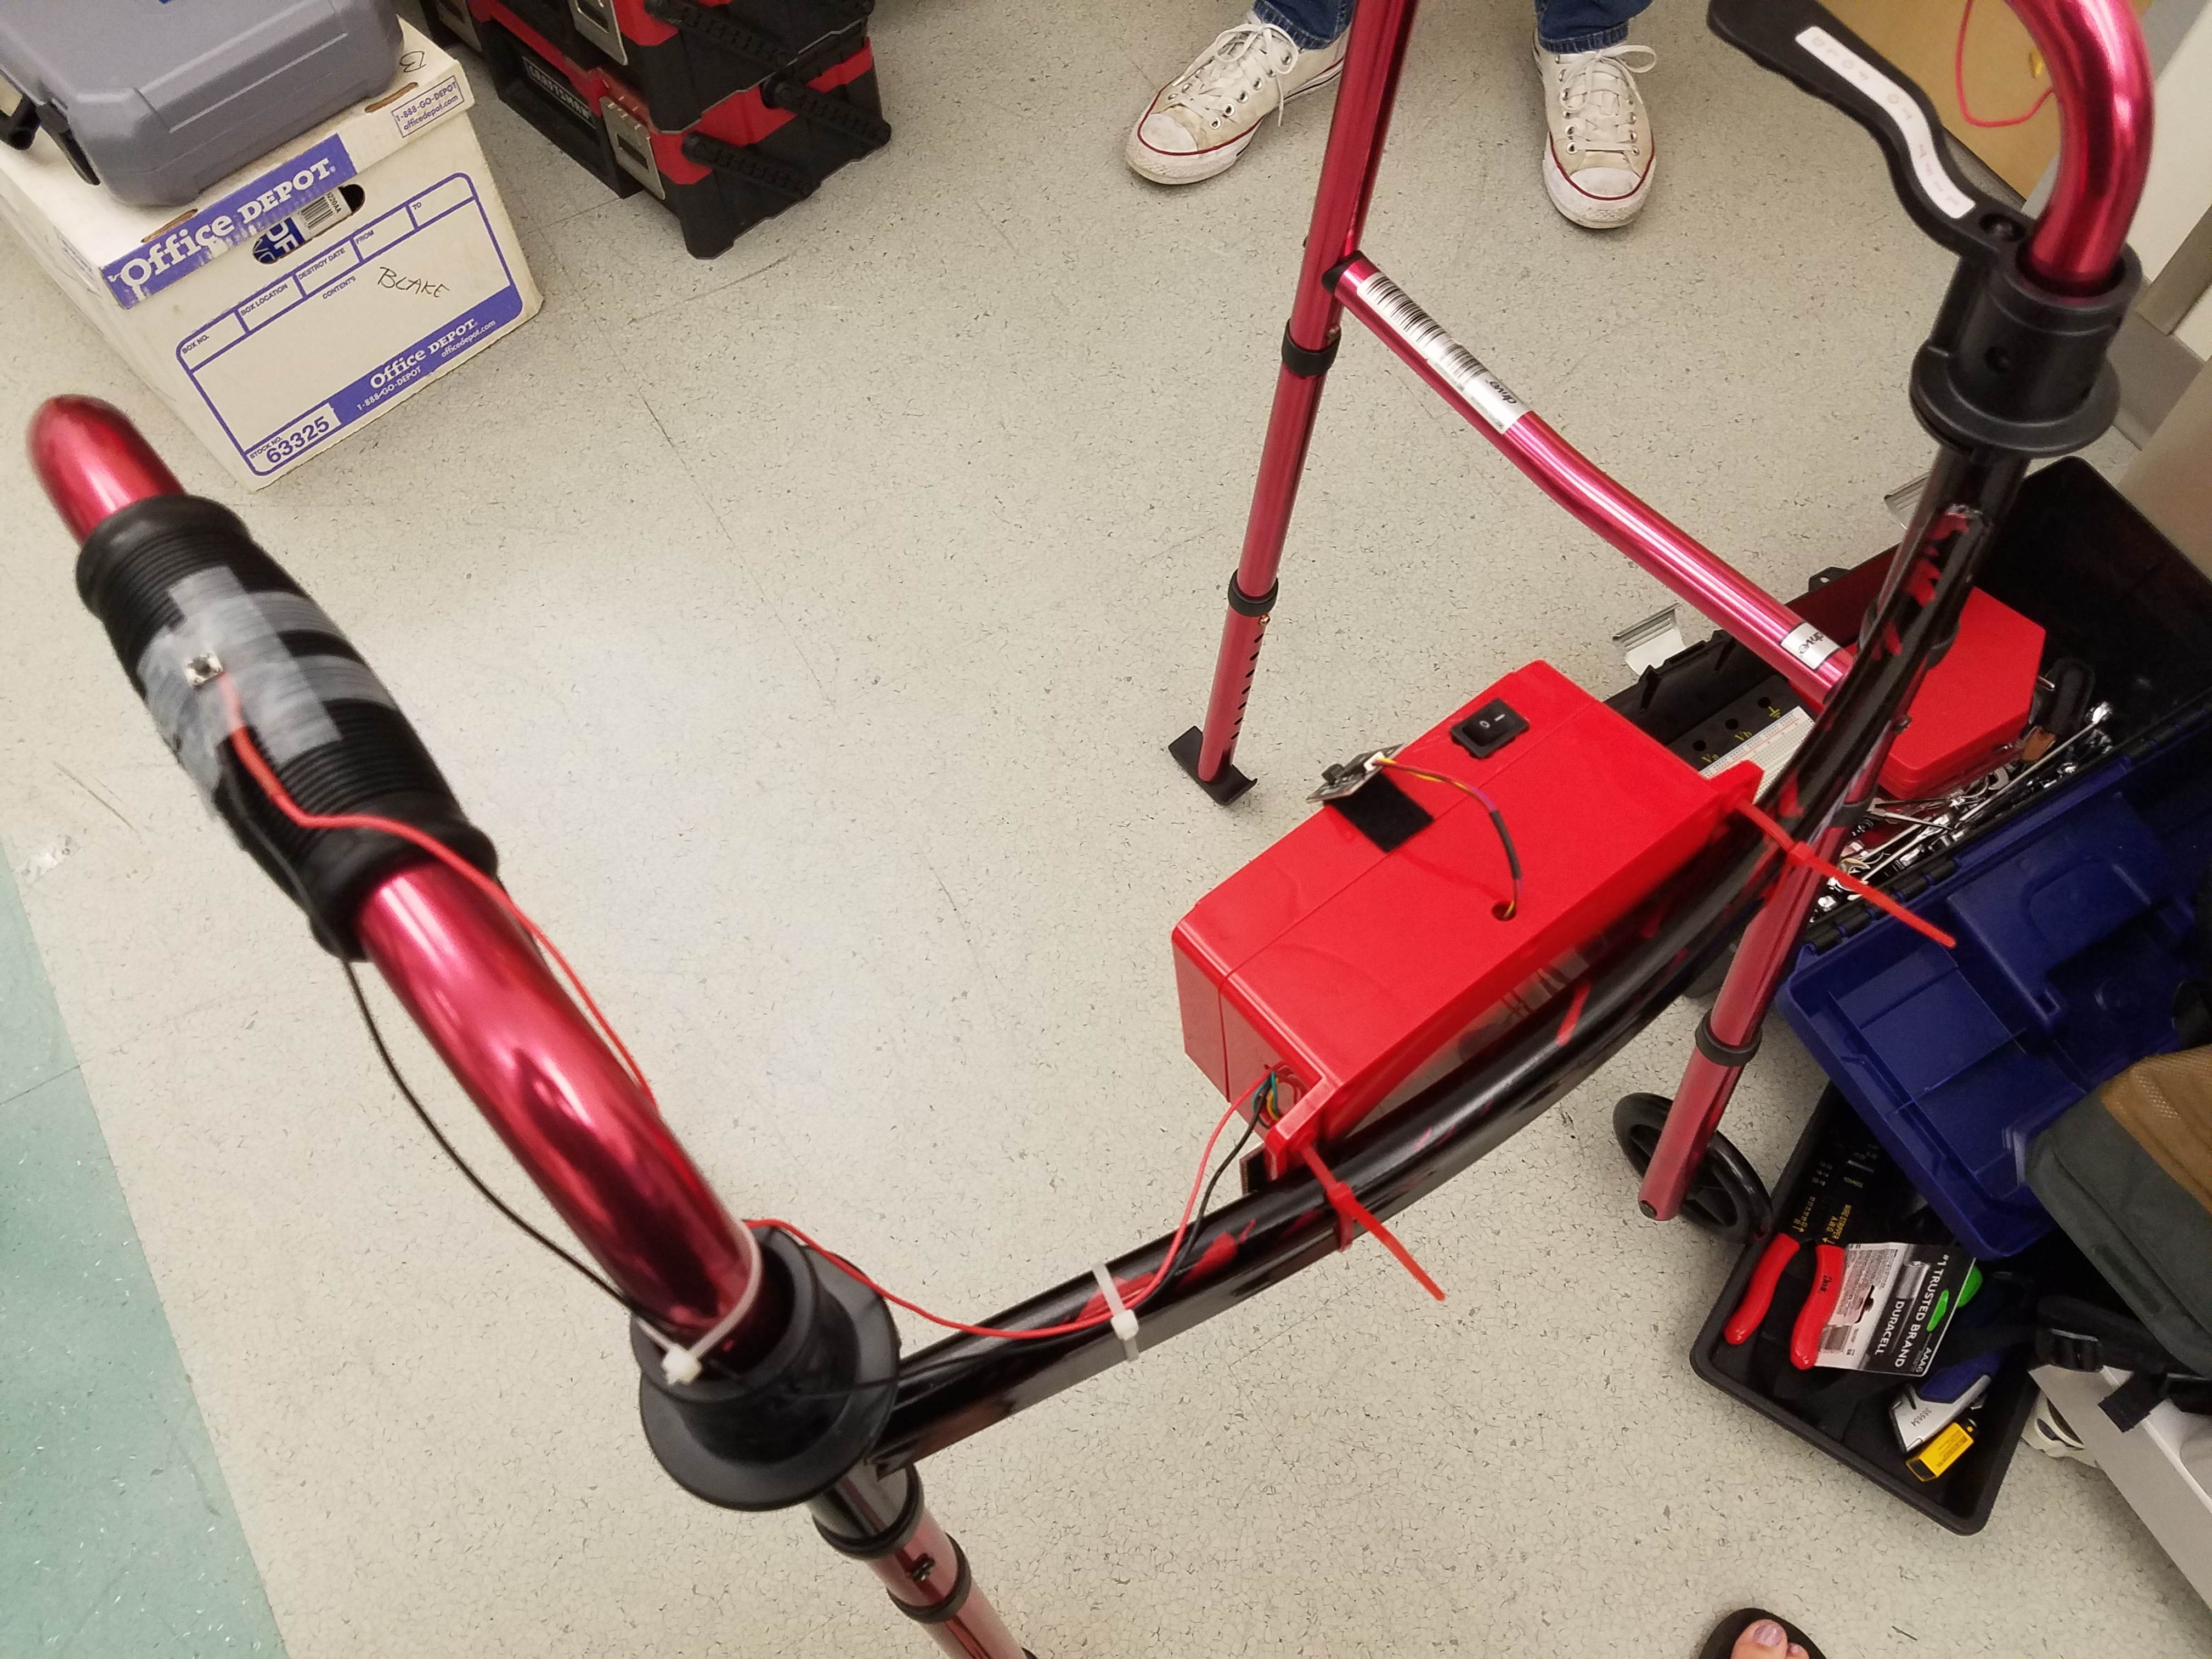
\includegraphics[width=.6\textwidth]{./images/complete_walker.png}
	\end{minipage}

\end{figure}

\begin{itemize}
	\item \textbf{Arduino Mega 2650}
	\item \textbf{Upper Sensor} - Sparkfun Distance Sensor Breakout – RFD77402 (QWIIC)
	\begin{itemize}
		\item Detects human presence up to 2 meters with I$^2$C
	\end{itemize}
	\item \textbf{Lower Sensor} - Sparkfun OpenPIR
	\begin{itemize}
		\item Measures for human presence and returns a digital 1 or 0 depending on whether some motion (ideally a human) is detected
	\end{itemize}
	\item \textbf{LEDs} - Sparkfun LP55231 LED Driver Breakout
	\begin{itemize}
		\item Interfaces with I$^2$C and three RGB LEDs for different colors and flashing
	\end{itemize}
	\item \textbf{Buttons} - Simple Momentary Push Buttons
	\begin{itemize}
		\item can be read with GPIO digital pins
		\item very noisy and require debouncing circuitry
	\end{itemize}
	\item \textbf{SD Card Module} - Sparkfun Level Shifting microSD Breakout
	\begin{itemize}
		\item Allows for mass storage of data on the Arduino Mega
	\end{itemize}
	\item \textbf{Real Time Clock (RTC) Module} - Real Time Clock (QWIIC) – RV-1805
	\begin{itemize}
		\item Maintains accurate date and time for logging
	\end{itemize}
	\item \textbf{QWIIC Adapter} - allowed for the 4 wires used for I$^2$C (SDA, SCL, 3.3V, GND) to be combined into a single solderless cable structure.
	
\end{itemize}




\section{Software Design}
The software for this project was all written in the Arduino IDE. Much of it was taken from example sketches, specifically the setup of sensors and peripherals. The libraries for all of the main functions are included in the libraries/ folder in the GitRepository. The software design main loop was built with the idea of being compatible with an app later on for monitoring. This app was furnished with Arduino compatibilty by Blynk, an Internet of Things (IoT) company based on creating solutions that the user can control from his/her phone. The main blynk documentation can be found by clicking \href{https://docs.blynk.cc/}{here.}

To go along with the modular approach to this design, the discrete components of the system are broken up into different files, unified by a common header \textit{definitions.h}.

\subsubsection{Blynk Disclaimer}
 Currently, the Blynk website uploading and writing to the phone breaks the system and freezes it, so that functionality is currently under investigation. In the meantime, that Blynk functionality is commented out. 

\subsection{Timing}
Before getting too deep into the code, it is important to bring up the issue of timing. Rather than using delays that could tie down the microcontroller, it would be far better to use timers that run specific functions at certain intervals. For this reason we use a \textbf{BlynkTimer}, something very similar to a simple timer created to be compatible with the Blynk system, and theoretically would prevent timing issues (which it didn't). This timer is an object that can have up to 10 different intervals and callbacks that can be set with the \textbf{setInterval()} command. The developer has the option of setting the interval, which should be long enough to not tie down the microcontroller, but short enough to allow for the accurate polling of the sensors. 

It's also important to note that in the code, not every sequence has to be complete or run every time the function is called. We add static integers and case statements to have the desired functionality without over-burdening the system. These are explained in detail as they arise. 

\subsection{Header file definitions.h}
The header file contains all of the information that applies to multiple files. This allows for the functions to be more readable and less cluttered if things are moved around. It also includes all other file inclusions that are necessary, globals, and pin declarations. Ideally, if one person was looking to hook up all the wires in the system correctly, they would only need to look at the header file. 

In addition to this information, it includes many of the module or object declarations that are used later on in the programs. These include things like the ledChip declaration. It is important to note that the ledChip and ledChip2 objects that are declared have numbers associated with them. These are the specific I$^2$C addresses that allow them to operate separately from one another. If one wants more information on this specifically, they can look at the led chip driver hookup guide \href{https://learn.sparkfun.com/tutorials/lp55231-breakout-board-hookup-guide/all}{here.} 

Finally, there are several global constants or other important information located in the header. One of the most important is the global \textbf{CARD\_OK}. This global can toggle wether an SD card is detected and allow the system to continue operation regardless of whether one is detected or not. While this is not necessary, If an SD card is not inserted, it is recommended to set this value to 0. Also the names of the states for the state machine are enumerated here, as well as the current state and next state. This allows functions from the button interrupts, for example, to change the value of next state even while it is in a separate file. The entire header file can be found in Listing~\ref{code:header} on Page~\pageref{code:header}.

\subsection{Main}
Based on a Blynk Example sketch for the ESP8266 WiFi chip on the WiFi shield, the main loop of the software function is designed to be as simple as possible. As with all Arduino main functions, there is a \textbf{setup} function and a \textbf{loop} function. The full main code is found in Listing~\ref{code:main} on Page~\pageref{code:main}. 


\subsubsection{The Setup}

The setup function is executed once at the beginning or upon reset, and then the loop function is run indefinitely. The setup is shown below in Listing~\ref{code:mainsetup}. Since the main loop hasn't been entered, delays are allowed here to make sure that Serial ports are set and any protocol or setup is taken care of correctly. All of the delays are kept small, however, to keep the Up-Time as short as possible, because there is a fair bit of handshaking that has to happen. Additionally, a lot of the specifics for the setup are kept out of this loop and are done in the individual files. Each of these functions in their entirety are in the Appendices in Full Code. 

\begin{lstlisting}[caption={The Main Setup}, label={code:mainsetup}]
void setup()
{
	// Debug console
	Serial.begin(9600);
	
	delay(10);
	
	// Set ESP8266 baud rate
	EspSerial.begin(ESP8266_BAUD);
	delay(10);
	
	// setting up function calls via the timer 
	// first argument is the duration between events in milliseconds 
	// up to 16 timers per timer object. 
	// max data sending rate of 10 values per second
	timer.setInterval(STATE_MACH_INTERVAL,StateMachine); // this is the timer that calls the state machine every STATE_MACH_INTERVAL miliseconds
	timer.setInterval(LED_INTERVAL,LEDMain); // can be on a separate time from the state machine if flashes must occur slower or faster 
	
	// WIFI Manager Attempts 
	// one-time thing: 
	//wifiManager.resetSettings(); 
	// setting up the auto connnect using WiFiManager Library
	//wifiManager.setConfigPortalTimeout(180); // waits 3 minutes and then will shut off. 
	//wifiManager.autoConnect("RemindME Walker","remindme"); 
	
	SetupLEDs(); 
	SetupRTCandSD();   
	SetupSensors(); 
	SetupButtonInterrupts(); 
	//Blynk.begin(auth, wifi, ssid, pass);
	SetupLEDDriveCurrents(); 
	ClearLED(); 
	DEBUG.println("Setup Complete!"); 
}
\end{lstlisting}


\subsubsection{The Loop}
The loop, as specified, is shown below in Listing~\ref{code:mainloop}. As one can see, it has been kept as simple as possible. Ideally, only the timer and Blynk would be run in the main loop, however, there were some functions that had to occur frequently: the updates from the real-time clock module (RTC) and monitoring if the SD card is currently inserted. 

\begin{lstlisting}[caption={The Main Loop}, label={code:mainloop}]
void loop()
{
	//Blynk.run();
	timer.run(); 
	if (rtc.updateTime() == false) //Updates the time variables from RTC
	{
		Serial.print("RTC failed to update");
	}
	// periodically checking 
	// currently disabled to prevent the SD card from preventing other operation of the device.
	
	// FIXME: maybe add a parameter that enables easier checking and initialization if possible
	if (!digitalRead(cardDetect))
	{
		initializeCard(); 
	}

}
\end{lstlisting}

\subsection{State Machine}
This state machine is based off of the Activity Diagram shown in Figure %find the figure number and insert the figure 
The state machine function, called every 100 ms as specified in \textit{definitions.h}, is shown in Listing~\ref{code:statemachcallback}. Like most state machines, this is implemented using a case statement. Each state has a dedicated function that carries out the operations of that state, whether it is monitoring, displaying LED output, or logging data. The full \textit{State\_Functions.ino} file can be found in Listing~\ref{code:StateMach} on Page~\pageref{code:StateMach}. 

\begin{lstlisting}[caption={The State Machine Callback Function}, label={code:statemachcallback}]
void StateMachine()
{ 
	static int counter = 0; 
	static unsigned long time_elapsed = 0; 
	counter = counter + 1;
	time_elapsed = counter * STATE_MACH_INTERVAL;  
	
	if(next_state != current_state) {
		//DEBUG.println("State change! Counter Reset"); 
		DEBUG.print("Current State: "); DEBUG.println(next_state); 
		counter = 0; 
	}
	// to account for if next_state was changed during the time interval, we switch right here
	current_state = next_state; 
	
	switch(current_state) {
		case waiting: 
		next_state = WaitingState(time_elapsed,&counter); 
		break; 
		case iAmHere: 
		next_state = IAmHereState(time_elapsed,&counter); 
		break; 
		case gentleReminder: 
		next_state = GentleReminderState(time_elapsed,&counter); 
		break;
		case strongReminder:
		next_state = StrongReminderState(time_elapsed,&counter); 
		break; 
		case thankYou: 
		next_state = ThankYouState(time_elapsed,&counter); 
		break;
		case inUse:
		next_state = InUseState(time_elapsed,&counter);
		break;
		default: 
		DEBUG.println("Error occured in the state diagram."); 
		break;     
	}

}
\end{lstlisting}

Each of the states, with its correct enumerated name, is elaborated a little further here below: 

\begin{itemize}
	\item \textbf{waiting}: the initial state, this is where the walker is scanning for human presence on either sensor. It checks the lower sensor every time, since it is a constant digital output on the PIR. The upper sensor is only checked every 2 seconds by comparison. 
	\item \textbf{iAmHere}: this state is gone to when either sensor detects some movement in front of it. The output is a white LED powerup sequence that reminds the user that it is there to be used. If a "proximal" signal, meaning the user could reach out and grab the walker, is detected from the upper sensor, the system moves to gentle reminder. 
	\item \textbf{gentleReminder}: this state is a sequence of repeating yellow lights in an effort to have the user to grab the walker without a sterner reminder. If this state isn't observed, the state can either go to strongReminder if we believe the user is ignoring the walker or still near, or the state can go to waiting if the user hasn't moved. 
	\item \textbf{strongReminder}: this state is a stronger flashing of red lights, eventually to be accompanied with an alarm that strongly suggests the user use the walker. If this warning is not observed after some amount of time, or the user has moved out of the way, then the state machine goes back to waiting. 
	\item \textbf{thankYou}: this state is triggered when one of the handles has been grabbed. It can only be reached from one of the interrupt handlers from the button external interrupts. It goes through a pleasant green light sequence and records the time of the user grabbing the walker to the SD card. After this has been completed and the sequence ends, the state machine always goes to inUse. 
	\item \textbf{inUse}: this state is used when either of the buttons is actively being pressed. If the person takes both hands off of the walker, the system goes to gentleReminder to remind the user to put their hands on the walker. 
\end{itemize}

%talk about the timing stuff. 
\subsubsection{Timing and Sequence Management in States}
Since we use the timer to call the state machine function, the scope of the state machine is not passed any information about what time it is, or what state is was in earlier. Due to reccomendations about avoiding the millis() function, static integers, which retain their value when the function returns, were used to remedy the problem. There is a static counter variable \textsl{counter} that increments by 1 each time the function is called. And since the timer interval is known, one can calculate how much time has elapsed since we entered the state. From there, the \textsl{time\_elapsed} is passed to the corresponding state functions. The counter is also passed in case the function resets the counter at any point. This is used in waitingState and inUse specifically to avoid getting massive counter integers that could wrap around. Otherwise, it's not currently muched used, but gives a lot of flexibility about how to manage time. The same basic time management scheme is used in the LED state to allow for sequences to occur in the same state. If interested to see the exact implementation, it is provided in the \textit{LED\_Functions.ino} file in Listing~\ref{code:LEDFunctions} with the counter and function calls in the \textit{LED\_Driver.ino} file in Listing~\ref{code:LEDDriver}. 

It is important to note at this point that whenever the state changes, \textbf{the counter is reset to 0}. 

\subsection{Sensors}
The sensor setup and functionality is largely taken care of the libraries that have been included. For the software, the sensors are simply black boxes, with functionality shown below:
\begin{itemize}
	\item Lower Sensor: detects motion and outputs a 1 if detected. outputs a 0 otherwise upon measurement. 
	\item Upper Sensor: detects distance. Outputs 2 if the user could grab the walker (about 1 meter away), outputs a 1 if the person is nearby (about 1-2.5 meters), and outputs 0 otherwise. 
\end{itemize}  
The RF sensor and OpenPIR sensor are configured via the functions to do exactly this. In addition, any setup necessary should happen in the \textbf{SetupSensors()} function called in the setup loop.

In addition, the buttons are technically sensors, so they have been included in this file. The interrupts are enabled in the setup as well, and then in the callback they set the next state to \textsl{thankYou}. The entire file is found in Listing~\ref{code:SensorFunctions} on Page~\pageref{code:SensorFunctions}

\subsection{LEDs}
The LEDs are broken up into two files: one that is entirely modular and independent of the LEDs used called \textit{LED\_Drivers.ino} (Listing~\ref{code:LEDDriver})and one that is hardware dependent and called \textit{LED\_Functions.ino} (Listing~\ref{code:LEDFunctions}). The independent file is formatted very similarly to the State Machine Callback, as it requires the same basic functionality. It calls state-specific functions that will do the sequences described above. Then the hardware dependent file goes and implements these. Depending on the time elapsed, the LEDs could be turning on or off, so there are sequence steps that are iterated through using a case statement. A simple example of one is reproduced below in Listing~\ref{code:ledfunc}. As one can see, depending on the counter value which is static like earlier, the LEDs will either turn on (by specifying a duty cycle of 50 out of 255) or turn off (by specifying a duty cycle of 0) and reset the counter to begin the cycle again. The duty cycle is much less than the maximum to save power, and since that brightness was found to be sufficient in indoor situations. 

\begin{lstlisting}[caption={The Strong Reminder LED function}, label={code:ledfunc}]
void StrongReminderLED(int * counter)
{

	switch(*counter){// this switch statement allows the same function to be called at a timer instance but have different results. 
		case 1: 
		ledChip.SetChannelPWM(redLED1,50);  // turn on
		ledChip.SetChannelPWM(redLED2,50);  // turn on
		ledChip.SetChannelPWM(redLED3,50);  // turn on
		ledChip2.SetChannelPWM(redLED1,50);  // turn on
		ledChip2.SetChannelPWM(redLED2,50);  // turn on
		ledChip2.SetChannelPWM(redLED3,50);  // turn on
		break;
		case 2: 
		ledChip.SetChannelPWM(redLED1,0);  // turn off
		ledChip.SetChannelPWM(redLED2,0);  // turn off
		ledChip.SetChannelPWM(redLED3,0);  // turn off
		ledChip2.SetChannelPWM(redLED1,0);  // turn off
		ledChip2.SetChannelPWM(redLED2,0);  // turn off
		ledChip2.SetChannelPWM(redLED3,0);  // turn off
		*counter = 0; // by setting it to 0 we get 1 the next time it comes around 
		break;
	}

}

\end{lstlisting}

\subsection{Real Time Clock Module}
The Real Time Clock Module (RTC Module) is a battery powered oscillator that can continue to hold an accurate time after the system has turned off. It also has a very nice library that works alongside it. The real-time clock has a straightforward setup and then can get a Date string as well as a Time string. The specific functions and how they are used in \textbf{PrintDateandTime()} are found in Listing~\ref{code:SDandRTC} on Page~\pageref{code:SDandRTC}. 

\subsection{Micro SD Card and Data Logging}
The micro SD card used uses a shifting $\mu$SD sparkfun board that uses Serial Peripheral Interface (SPI) protocols unlike the rest of the boards I$^2$C. It is additionally able to continually check for the presence of an SD card, but also operate without one should the need arise. There is a nice library for this as well available, that was cannibalized to fit the needs of this project. The micro SD card should work directly out of the box, but if it does not then there is searchable documentation to format it appropriately. 

Additionally, since there was not one perfect way to save files, and one years worth of files would have been excessive, we decided to break files into week intervals. Each text file would start on Sunday of a given week of the year and be named the year, the word week, and then the week of the year: \textit{19week12.txt}. This is implemented using the \textbf{PrintDateandTime()} function, which proceeds to put this onto the SD card. This card can then be plugged into most computers using a micro-SD to SD card adapter and read easily. 

One can also use \textbf{PrintDateandTimeVerbose()} For additional information about the specific day, although this is unnecessary. In future iterations, the specific logging and methods used may need to change, so this should act more as a framework than a final solution. The full code is located with the RTC Module code in Listing~\ref{code:SDandRTC} on Page~\pageref{code:SDandRTC}.

\subsection{Future Software Directions}

As aforementioned in the Blynk Disclaimer is the WiFi, while implemented in hardware, was not fully able to be utilized. The ability for the WiFi to be connected via a soft access point so that the end user doesn't have to do any coding is also a final product must-have. Additionally, the WiFi had data transfer problems, and would freeze up the state machine. Fixing that is a top priority in future endeavors, and there are a couple possible solutions to help this problem:
\begin{itemize}
	\item Take other functions out of the main loop
	\item Extend timing periods for the state machine
	\item Look into disabling the SPI (SD card) and see if that makes the transfer easier
	\item Change the buttons from interrupt to polling
	\item Look into other alternatives to Blynk, which may require more work or an html page
\end{itemize}

Another issue is the button triggers. Even with a debouncing circuit, there is still a significant amount of noise from the interrupts. Potentially this response could be better debounced by simply polling the levels, since that is the quickest that the information could be acted on. Additionally, freeing up external interrupts, as mentioned, could solve some of the WiFi connection problems. 

Additionally, we would like to add the library for a speaker, once available, and have different files or tones associated with different states:
\begin{itemize}
	\item A power up sound for iAmHere
	\item A mild bong for gentleReminder
	\item A strong buzzer sound or words for strongReminder
	\item A pleasant wind down note for thankYou
\end{itemize}

Since the thank you state song should be at least somewhat pleasant, we think we may want to have mp3s saved to the device to play on a small speaker. This could be something the end user has the ability to upload to the same SD card that is logging the data. 

Additionally, we tried to keep a consistent serial DEBUG that was separate from the Basic Serial, in case someone wanted to monitor on Serial2, for instance (currently it is set to serial 1 and there is no difference between DEBUG.println and Serial.println). In future versions, however, we'd like to be able to comment out the DEBUG definition and have those prints not work, which would require wrapping those print statements in an if statement (may attempt to implement in Notepad ++ with a find and replace of some sort).


\section{Results and Lessons Learned}
Apart from the Wifi Sensor and the Speaker, most of the project worked flawlessly, we sometimes had issues with the button interrupts not working perfectly and the system thinking they were constantly on. This could be fixed with better buttons and possibly switching to polling the buttons. The root cause requires further investigation. 

The state machine and sensors worked very well together, and proved to streamline the thought process. Splitting key components into separate folders also worked very well.  

If we were to start over with this project, we probably would have had a much more formal design process to integrate system components, moving from the Uno to the Mega beforehand. Additionally, we would have started with Blynk from the beginning and not tried to get the wifi shield to work through other methods which took a lot of time. 



\section{System Setup Instructions}
% put the libraries of the Arduino tab into the Arduino documents folder thingy
The git hub repository where all of the code written for Arduino is kept, and can be cloned using \href{https://github.com/langley2119/Embedded_System_SmartWalker.git}{this address}. 


To begin using the software, one needs to load the libraries into the Arduino IDE. The IDE has a specific \textsl{libraries} folder, likely in Documents/Arduino/ that must include the libraries. Rather than adding all of the libraries from the Library Manager or trying to add zip files individually, we recommend \textbf{Copy} and \textbf{Pasting} the libraries/ Folder included in the repository directly to the Arduino folder. This saves a lot of time searching for the exact libraries. Additionally, one can now open the code from where the user has the repository and make all his/her changes there if desired, for easier file management.  

From here one should be able to select the mega 2560 as the desired board to build on and find the correct COM port and upload successfully. The code can be easily modified in the IDE and this is where we primarily did our development.

\subsection{Serial Communication and Debugging}
To debug certain steps, the development team would often send outputs - such as the state or when a specific loop had been entered - to the serial output. This can easily be read from the Serial Monitor inside of the IDE, and gives some sense of what is going on in the system. This was immensely helpful as we continued developing, and some of the more important messages we have left un-commented, so the user can see the progression. However, there are many messages that have been commented such as the sensor outputting distance, which a future developer is free to un-comment and check. 

\subsection{A note when working with Libraries and the Mega}
Unfortunately, the pinouts on the Arduino Uno and Arduino Mega are very different, and most libraries are written for the Uno. This means that a library that may work flawlessly on the Uno has partial or no functionality on the Mega. The development team would often have to change pins in the system (such as the primary SDA and SCL pins, and the SPI pins) to get the system to function correctly. The transition from Uno to Mega often required pinout information found on the Arduino websites.

It is therefore recommended to get the library and basic functionality desired starting on an Uno, and then migrate the technology to the Mega. This can ease a significant amount of frustration as a working system has already been established. 

\section{Conclusion}
The smart walker project as it sits currently is a significant step in the right direction to help elderly people who are required to use a walker. It is, however, by no means finished. With the WiFi and the speaker notable omissions, there is still a non-trivial amount of work left on the project to complete this stage of the prototype. From here, we hope that future developers can design a more complete PCB layout, design a custom housing, and make this product reach market shelves.

\section{Appendices}
Listed below is the entire code used in the project, as well as links to many of the components and other helpful information. 
\subsection{Full Code}

\Cpp{Header File} {code:header} {../ESP8266_Shield_example_minus_connman/definitions.h}

\Cpp{Main Arduino Code} {code:main} {../ESP8266_Shield_example_minus_connman/ESP8266_Shield_example_minus_connman.ino}

\Cpp{The State Machine and Associated Functions} {code:StateMach} {../ESP8266_Shield_example_minus_connman/State_Functions.ino}

\Cpp{The LED Drivers} {code:LEDDriver} {../ESP8266_Shield_example_minus_connman/LED_Drivers.ino}

\Cpp{The LED Functions} {code:LEDFunctions} {../ESP8266_Shield_example_minus_connman/LED_Functions.ino}

\Cpp{The SD card and RTC functionality} {code:SDandRTC} {../ESP8266_Shield_example_minus_connman/SD_save_files2.ino}

\Cpp{The Sensor Functions} {code:SensorFunctions} {../ESP8266_Shield_example_minus_connman/Sensor_Functions.ino}

\subsection{URL References}
\begin{itemize}
	\item Git Hub Repository: \url{https://github.com/langley2119/Embedded_System_SmartWalker.git}
	\item BLYNK Main Document: \url{https://docs.blynk.cc/}
	\item LED Hookup Guide:  \url{https://learn.sparkfun.com/tutorials/lp55231-breakout-board-hookup-guide/all}
	\item Upper Sensor (current version) \url{https://www.sparkfun.com/products/14539}
	\item Lower Sensor \url{https://www.sparkfun.com/products/13968}
	\item microSD breakout \url{https://www.sparkfun.com/products/13743}
	\item LED Breakout Driver: \url{https://www.sparkfun.com/products/13884}
	\item RTC Module (retired): \url{https://www.sparkfun.com/products/retired/14642}
	\item RTC Module (QWIIC compatible and current) \url{https://www.sparkfun.com/products/14558}
	\item Enclosure: \url{https://www.sparkfun.com/products/11366}
	\item QWIIC Adapter: \url{https://www.sparkfun.com/products/14495}
\end{itemize}

\subsection{Labed System}
\begin{figure} [h]
	\begin{center}
		\caption {The Labeled System} \label{fig:labels}
		\includegraphics[width=\textwidth]{./images/LabeledSystem.png}
	\end{center}
\end{figure}

\end{document}